\subsection{题目描述}
\noindent Derive the five-point formula for the second-order derivative.

\subsection{解答}
利用函数 \( f \) 在点 \( i \pm k \) 处的泰勒展开,得到以下差分表达式:

\[
\begin{aligned}
f_{i+2} &= f_i + 2 h f_i' + 2 h^2 f_i'' + \frac{4 h^3}{3} f_i''' + \frac{2 h^4}{3} f_i^{(4)} + \frac{8 h^5}{15} f_i^{(5)} + \mathcal{O}(h^6), \\
f_{i+1} &= f_i + h f_i' + \frac{h^2}{2} f_i'' + \frac{h^3}{6} f_i''' + \frac{h^4}{24} f_i^{(4)} + \frac{h^5}{120} f_i^{(5)} + \mathcal{O}(h^6), \\
f_{i-1} &= f_i - h f_i' + \frac{h^2}{2} f_i'' - \frac{h^3}{6} f_i''' + \frac{h^4}{24} f_i^{(4)} - \frac{h^5}{120} f_i^{(5)} + \mathcal{O}(h^6), \\
f_{i-2} &= f_i - 2 h f_i' + 2 h^2 f_i'' - \frac{4 h^3}{3} f_i''' + \frac{2 h^4}{3} f_i^{(4)} - \frac{8 h^5}{15} f_i^{(5)} + \mathcal{O}(h^6).
\end{aligned}
\]

目标是构造一个线性组合以消除一阶导数 \( f_i' \)、三阶导数 \( f_i''' \) 及五阶导数 \( f_i^{(5)} \),不妨设:

\[
A f_{i+2} + B f_{i+1} + C f_i + D f_{i-1} + E f_{i-2} = K f_i'' + \mathcal{O}(h^6),
\]

通过匹配各阶 \( h \) 的系数,可以构建方程组,观察各系数,不妨设\( K = 12 \)并约分,改写为增广矩阵形式,并使用我们在\texttt{Assignment\_3/Problem\_2}中实现的高斯消元法解得(不出意外是行满秩的,有重复约束条件)
\[
\begin{pmatrix}
1 & 1 & 1 & 1 & 1 & | & 0 \\
2 & 1 & 0 & -1 & -2 & | & 0 \\
4 & 1 & 0 & 1 & 4 & | & 24 \\
8 & 1 & 0 & -1 & -8 & | & 0 \\
16 & 1 & 0 & 1 & 16 & | & 0 \\
64 & 1 & 0 & -1 & -64 & | & 0 \\
\end{pmatrix}
\rightarrow
\begin{pmatrix}
A \\
B \\
C \\
D \\
E 
\end{pmatrix}
= 
\begin{pmatrix}
-1 \\
16 \\
-30 \\
16 \\
-1
\end{pmatrix}
\]

\begin{figure}[H]
    \centering
    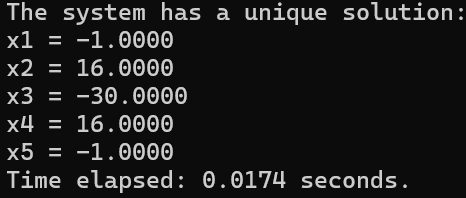
\includegraphics[width=1.0\textwidth]{Problem_1/figs/coeff.png}
    \caption{运行结果}
\end{figure}
因此,求二阶差分的五点公式为:

\[
- f_{i+2} + 16 f_{i+1} - 30 f_i + 16 f_{i-1} - f_{i-2} = 12 h^2 f_i'' + \mathcal{O}(h^6),
\]

即,

\[
\boxed{ f_i'' = \frac{ -f_{i+2} + 16 f_{i+1} - 30 f_i + 16 f_{i-1} - f_{i-2} }{12 h^2} + \mathcal{O}(h^4) }
\]



